\section{A Second Method of Distributing the Chronocratorship with Respect to the Rising Times of the Signs and the Periods of the Stars (2K,3P)}

\textbf{/267K/} Since the overall chronocratorships and their mutual relationships have been determined, I will now append the detailed distribution which I derived with much experience and toil. In advance I urge all those who wish to strive for the best, and particularly our followers (or any of those who have the incurable, longstanding
disease of scholarship), to go soberly in the matter of methods, \textbf{/255P/} and never to forecast carelessly using any system. For often one distribution when it takes effect indicates a good chronocratorship—and indeed it will be good if it controls the chronocratorship by itself. If, however, another chronocratorship of malefics takes effect, it not only turns away the good but becomes a cause of evil. In such a case, even if the chronocratorship of benefics is vigorous in the nativity, the activity and rank will come accompanied by reversals and losses. If the chronocratorship of malefics is strong,
unemployment, penalties, and upheavals will occur until the chronocratorship of benefics is operative.

Moreover, often a star which is in a given sign, which is completing its own period or the time-interval $<$=rising time$>$ of the sign, and which is apparently passing out of its time as chronocrator, combines with another star and becomes the cause of a different outcome or continues to keep the nativity in the same condition. In addition, the sextile aspects must be taken into consideration, because they are powerful and beneficial, particularly when they alone are operative. 

For infant nativities, it is necessary to calculate the chronocratorships of the stars in aspect using first the days, then the years. As examples let us append nativities which we have tested with precision in some forecasts and which I had a hand in: \Sun, \Moon, \Mercury\xspace in \Sagittarius, \Saturn\xspace in \Cancer, \Jupiter, Ascendant in \Scorpio, \Mars\xspace in \Capricorn, \Venus\xspace in \Aquarius, Lot of Fortune in \Scorpio, klima 2\footnote{\textit{Greek Horoscopes} dates the chart to December 8, 120 CE abour 4 a.m.}. 

\begin{wrapfigure}[14]{R}{7cm}
\centering
\vspace{-20pt}
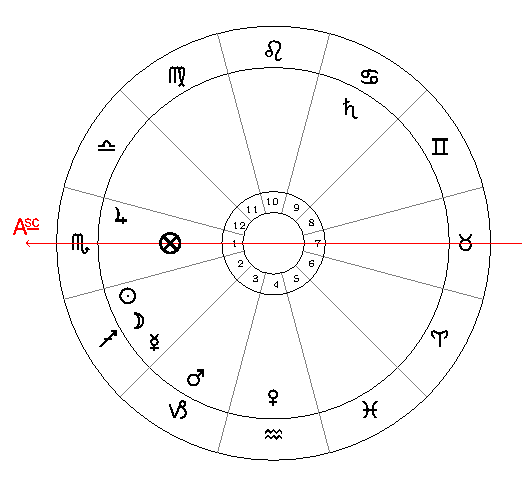
\includegraphics[width=.68\textwidth]{charts/7_3_1}
\caption{Chart 73 [VII.3.1, GH L120, XII]}
\label{fig:chart73}
\end{wrapfigure}

In his 33rd year he was exiled: the rising time $<$33$>$ of \Cancer\xspace in which \Saturn\xspace was located with \Mars\xspace in opposition. The \Moon\xspace \Sextile\xspace to
\Venus\xspace indicated treachery from female individuals during the 33rd year. He was also in danger in his 27th year because of \Capricorn\xspace and in his 30th and \textbf{/268K/} 40th years because of bodily illnesses of the eyes and feet: the period of \Cancer $<$=\Moon$>$ is 25 and of \Mars, which was in opposition, 15. Until his 42nd year the period of \Mars\xspace and the rising time of \Capricorn\xspace $<$27$>$ were also operative, and in this time many crises arose. 

You see that in such configurations it is necessary to forecast after determining the $<$degrees$>$, in order to see if some ray of the benefics may take effect and may remove most of the bad effects.

\newpage
Another example: \Sun, \Venus\xspace in \Libra, \Saturn\xspace in \Aries, \Jupiter\xspace in \Taurus, \Mars\xspace $<$in \Libra$>$, \Mercury\xspace in \Virgo, \Moon\xspace in \Sagittarius, Ascendant in \Libra, klima 3\footnote{\textit{Greek Horoscopes} dates the chart to September 24, 114 at about sunrise}. 

\begin{wrapfigure}[14]{R}{7cm}
\centering
\vspace{-20pt}
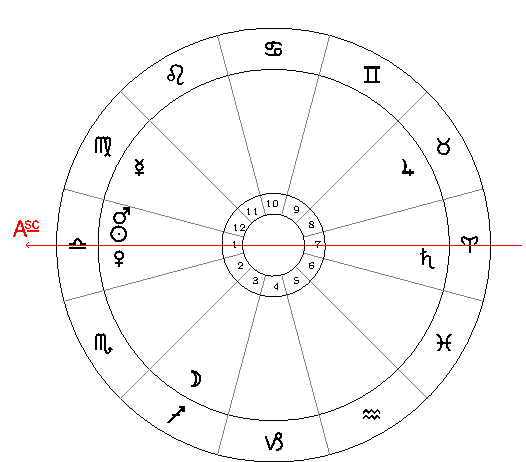
\includegraphics[width=.68\textwidth]{charts/7_3_2}
\caption{Chart 74 [VII.3.2, GH L114, IX]}
\label{fig:chart74}
\end{wrapfigure}

In his 39th year he was exiled: the rising time of \Aries\xspace is 20, and \Saturn\xspace is there with the \Sun\xspace (19) in opposition. Both were in opposition to their own exaltations. To be sure, he had critical periods in the previous years, but \textbf{/256P/} we observed the 39th year because of the comparison with the preceding nativity, which was his brother’s. We must marvel at the natural law that brought the chronocratorships to the same results, even though they were born in different klimata.

\newpage
Another example: \Sun, \Mercury, Ascendant in \Sagittarius, \Moon\xspace in \Cancer, \Saturn\xspace in \Leo, \Jupiter\xspace in
\Capricorn, \Mars\xspace in \Aquarius, \Venus\xspace in \Scorpio, klima 2\footnote{\textit{Greek Horoscopes} dates the chart to December 4, 122 CE about sunrise}.

\begin{wrapfigure}[14]{R}{7cm}
\centering
\vspace{-20pt}
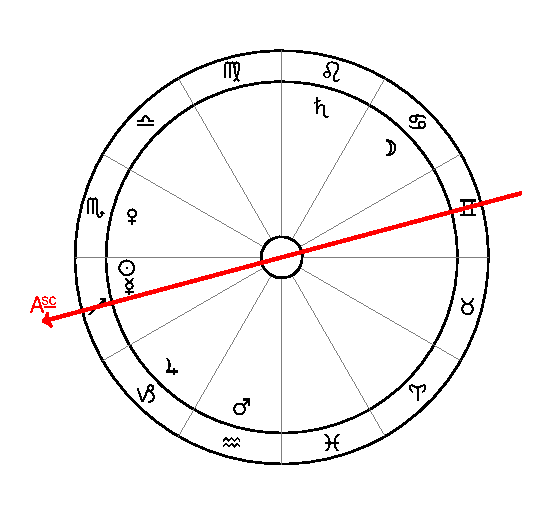
\includegraphics[width=.68\textwidth]{charts/7_3_3}
\caption{Chart 75 [VII.3.3, GH L122, XII]}
\label{fig:chart75}
\end{wrapfigure}


In his 34th year his wife died because of the 19 of \Leo\xspace $<$=\Sun$>$ and the 15 of \Scorpio\xspace $<$=\Mars$>$, or the 15 of \Mars\xspace itself, since both malefics hemmed in \Venus. 

In his 36th year he was about to go on trial, being accused before the king on a charge arising from the death of his wife, on the grounds that she had been treacherously murdered, but he fled into exile. For
36 is the rising time of \Leo\xspace and of \Scorpio\xspace as well, the location of \Venus, in inferior aspect with \Saturn. 

A more kindly chronocratorship was about to occur in his 37th year, because of the 12 of \Jupiter\xspace and the 25 of the \Moon, in opposition $<$to \Jupiter$>$. Many other factors were operative in the past and the future $<$chronocratorships$>$, but I have thought it necessary to set forth only those which I myself know exactly
and which I had a hand in.

\newpage
Another example: \Sun, \Mars, \Venus\xspace in \Sagittarius, \Moon\xspace in \Libra, \Saturn\xspace in \Gemini, \Jupiter\xspace in
\Virgo, \Mercury\xspace in \Scorpio, Ascendant in \Capricorn\footnote{\textit{[This chart was the second example chart given in Book II, section 36. GH dates it to November 12, 118 CE]}}.

\begin{wrapfigure}[13]{R}{7cm}
\centering
\vspace{-20pt}
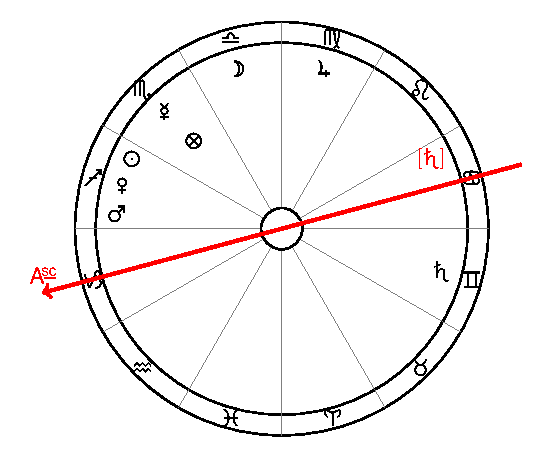
\includegraphics[width=.68\textwidth]{charts/2_36_2}
\caption{Chart 21a [VII.3.4, GH L118]}
\label{fig:chart21a}
\end{wrapfigure} 

In his 19th year his father died violently and he himself was blinded by eye trouble. In the same year he travelled abroad and was in danger at sea, because the \Sun’s period $<$19$>$ was operative, with \Mars\xspace in conjunction and \Saturn in opposition. 

In his 20th year he recovered his sight through a treatment and an ointment given by an oracle of the god. But \Saturn\xspace $<$in
\Gemini$>$ even then was operative, with \Gemini\xspace $<$=\Mercury$>$ giving 20, and therefore he suffered many ills.

\Virgo $<$=\Mercury$>$ also indicated 20, since \Jupiter was in that sign. \textbf{/269K/} The 20 came from the 12 of \Jupiter\xspace plus the 8 of \Venus\xspace square. The chronocratorship belonged to many stars, but the operative ones were powerful. The stars in conjunction or aspect have a weaker influence for helping or harming, but they do have some power, especially when (as we have mentioned before) they are in the sign or the exaltation of, or are trine with, a fellow sect-member. 

Benefics and malefics had the same effects since they were preceding the angles, but \Jupiter\xspace was most active since it was in the sign and $<$the IX Place of$>$ the God and of Foreign Lands. Additionally, they were found in signs of equal rising time or in houses of the same star $<$\Mercury$>$, and are as effective as if they were in aspect, particularly when the signs are found to be at
the angles or operative.

\textbf{/257P/} Another example: \Sun, \Jupiter, Ascendant in \Cancer, \Moon\xspace in \Sagittarius, \Saturn\xspace in \Gemini,
\Mars\xspace in \Taurus, \Venus, \Mercury\xspace in \Leo, klima 3\footnote{\textit{Greek Horoscopes} dates the chart to June 30, 117 CE about 2 p.m.}.

\begin{wrapfigure}[13]{R}{7cm}
\centering
\vspace{-20pt}
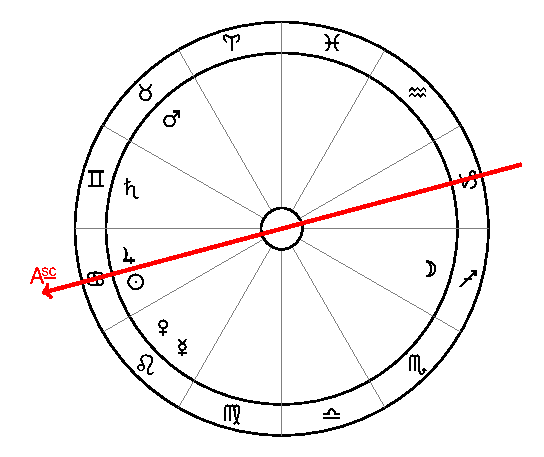
\includegraphics[width=.68\textwidth]{charts/7_3_5}
\caption{Chart 76 [VII.3.5, GH L117, VI]}
\label{fig:chart76}
\end{wrapfigure} 

After serving in a distinguished military post, he was involved in an accusation in his 38th year and lost his rank: the rising time of \Taurus, 23, and the period of \Mars, 15 were operative for a total of 38. In addition, the sextile configuration of \Saturn\xspace and \Venus\xspace totalled 38. Moreover, from his 37th year he endured enmities and reversals, because the \Moon\xspace indicated 25 and \Sagittarius\xspace $<$=\Jupiter$>$ indicated 12 for a total of 37, with \Saturn\xspace in opposition. On the other hand, \Cancer\xspace $<$=\Moon$>$ had 25 and \Jupiter\xspace 12, and as a result he got some small assistance. 

In his 39th year he was in a lawsuit and was imprisoned with no power to set things straight. For \Mercury\xspace in \Leo allotted 20
plus 19 for the sign $<$=\Sun$>$, but it was in inferior aspect $<$\Sextile to the left$>$ with the star which caused the crisis $<$\Saturn$>$ and hence was weaker. Besides, \Saturn\xspace was about to begin another period of setbacks: the rising time of \Gemini\xspace is 28 plus 12 for \Sagittarius\xspace $<$=\Jupiter$>$, for a total of 40. During this period the native traveled abroad and was betrayed through documents by a woman; he became debt-ridden and troubled about slaves, some because of alienation, others because of death and penalties. He himself was physically ill. Even though the chronocrators were malefic, some hint of good is about to appear from the benefics, and total loss and degradation will not follow. For friendships and hopes are being sown in advance, and it is through these that the native’s troubles are alleviated. In the same way, even if the chronocrators had been benefic, some malefic influence is about to impinge: the friendships change to enmity and the loss of livelihood comes quickly with the loss of standing accompanying it. 

If the stars in trine, sextile, or some other aspect are operative, and if \textbf{/270K/} another aspect does not interpose itself in the succeeding period, the original aspect will predominate. Again, if the same stars later become chronocrators, they will display the same influence on outcomes in the same activities or ranks, predominating until another influence is operative.

\begin{wrapfigure}[15]{R}{7cm}
\centering
\vspace{-20pt}
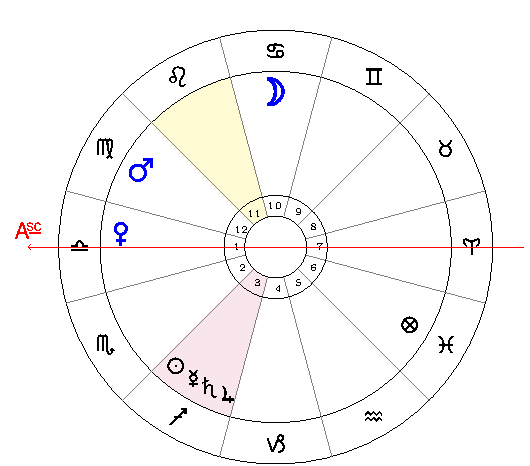
\includegraphics[width=.68\textwidth]{charts/2_21_5}
\caption{Chart 5a [VII.3.5, GH L74, XI]}
\label{fig:chart5a}
\end{wrapfigure} 

Another example: \Sun, \Saturn, \Jupiter, \Mercury\xspace in \Sagittarius, \Moon\xspace in \Cancer, \Mars\xspace in \Virgo,
\Venus, Ascendant in \Libra, klima 1\footnote{\textit{Chart was originally given as the fifth example in Book II, section 22}}.

In his 69th year he was judged worthy of the governorship and became feared and spectacularly respected. He was blessed by the public \textbf{/258P/} but was also hated, was involved in mob uproar and disturbances, and did not complete his term of office. He was overtaken by painful illnesses and death. Operative at the time were the rising time of Libra $<$Ascendant$>$, 38;20, and
that of \Cancer\xspace $<$MC$>$, 31;40, for a total of 69. The malefics happened to total the same length of time: 30 for \Saturn, 19 for the \Sun, plus 20 for \Mercury\xspace total 69, or in addition 38;20 for \Virgo $<$\Mars$>$, 12 for \Jupiter, plus 19 for the \Sun\xspace total 69. All the stars were operative and each of them had its own effects according to its own nature and its place in the natal chart.

That most of the stars—or even all of them—can be actively producing their effects at the same time can be observed from these examples. We find that activities take place throughout the cosmic fabric of the
earth every day and every hour: births, deaths, inheritances, ranks, ruins, injuries, illnesses, etc., whatever good or bad arises in man’s life. For the universe, whirling in a sphere and sending the emanations of the stars onto this globe, does nothing vainly or uselessly: every moment it makes many things new in life, things which each person must abide patiently, some at one time, others at another, in order to fulfill the aims of Fate.

Many men have devoted themselves to such matters and have compiled many books and many systems; indeed all of them have left many interminably long accounts for men. A comparison can be
made between them and those men who appear to be rich, but who in fact owe much money, and who leave little to their heirs. The heirs are well satisfied at first, although they receive as their own only a little money and have a very brief possession of the great wealth. (The fact of their ignorance \textbf{/271K/} casts a great delusion on them.) However, when they have become involved in lawsuits, troubles, and setbacks, because of the $<$attendant$>$ hatred and anxiety they choose to get rid not only of this useless inheritance,
but also of what they had enjoyed having. The same things happens to men who spend much time in the endless mass of treatises: they do not heal their chronic disease $<$curiosity$>$, but rather lose their minds, their education, and the profession which they already have.
For my part, I do not wall myself in with a show of words or a pile of books, but I have “embellished” my $<$treatise$>$ with conciseness and truth. As a result, my heirs enjoy their inheritance without lawsuits and hatred as long as they live, some progressing far in forecasting by means of careful and accurate study. Others who approach it on a part-time or a negligent basis gain \textbf{/259P/} little—except that
they do gain a higher and a better profit than those who study with great toil the interminable systems of others.

Since I myself have been a finder of treasures—and I have found not only the guarded topics, but have also illuminated the hidden topics—my readers must also be aware that, when delving deeply into them,
they have discovered what was mystically hidden in darkness. One who enrolls in my school must also know what basis his own horoscope has, and he must apply himself to forecasting after taking into account
his active chronocrators, so that he might gain profit or testimony $<$?$>$. (If he applies himself $<$to forecasting$>$ in the chronocratorship of a malefic, he blames the method when he fails through ignorance or the omission of some place.) Nevertheless, if he searches with accuracy, he will not fail of this gift, and he will be thought worthy of the honor that any of the “Lovers of Time” may show him, depending on the basis of his nativity. Since I have experienced these things in my own life, I have explained them.

Wherefore one should not blame me or the forecast for the chronocrators, but one should soldier on bravely and gladly under all circumstances, recognizing the level of one’s nativity. It is of no use to live in despair, wishing to equal the fortunes of other men. One must remember: 

\begin{verse}
Lead me, O Zeus, and you, O Fate, \\
Wherever you have assigned me to go. \\
I will follow unhesitating. If I did not wish,  \\
Having become base, I will suffer this anyway. \\
\end{verse}

/272K/ And this:
\begin{verse}
Fate wove with the strand of his birth that day he was born to his mother. $<$Iliad 19.128$>$
\end{verse}

And this:
\begin{verse}
But as for Fate, I thing that no man has yet escaped it. $<$Iliad 6.488$>$
\end{verse}

\newpage